\documentclass[tikz]{standalone}
\usepackage{tikz}
\usetikzlibrary{matrix,fit,backgrounds,calc,decorations.markings,arrows.meta,shapes.geometric}
\usepackage{amsmath}
\usepackage{braket}

\begin{document}
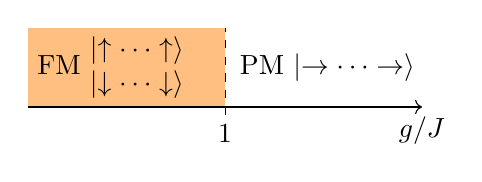
\begin{tikzpicture}[]
	\fill[fill=orange!50!white] (0, 0) rectangle (2.5, 1.);
	\fill[fill=white] (2.5, 1) rectangle (5, 0.);
	\draw[->] (0, 0) -- (5., 0) ;
	\foreach \i in {0..1}
	\draw[thin, dashed] (2.5,-.1) -- (2.5,1);
	\node[below] at (2.5,-0.1) {$1$};
	\node[below] at (5,0) {$g/J$};
	\node at (1.2,0.5) {FM \parbox{1.5cm}{$\ket{\uparrow \cdots \uparrow} \\ \ket{\downarrow \cdots \downarrow}  $}};
	\node at (3.8,0.5) {PM $\ket{\rightarrow \cdots \rightarrow} $};
	% \node[color=white] at (0,0) {$\mathbf{\ket{0}}$};
\end{tikzpicture}
\end{document}
